\documentclass[]{article}

\usepackage{graphicx}
\title{What even is data?}
\author{}

\begin{document}

\maketitle
\section{Let's Talk Data}
We hear and talk a lot about \textit{data} science or about large \textit{data}. But what really are \textit{ data}? What does it look like? Does it have a structure we can envision?Think about the problem of trying to predict the temperature of a certain point in the city on the following day. We know(somehow)that the temperature will depend on the temperature of that location the previous day ($T_{-1}$, the humidity(in percentage)($H_{-1}$)the amount of rainfall(in mm)($R_{-1})$ and whether the point is located within the city or outside ($loc\in \{0,1\},\{in,out\} $). The datapoint then in this case looks like the observed values for the tuple $( T_{-1},H_{-1},{R_{-1},loc})$.
If we are making $d$ observations, our datapoint will be a $d-yuple$. We conventionlly denote an observation/datapoint by $x$. We just saw that $x \in \mathbf{R^d}$.

\section{From data toDataset}
We usually collect multiple observations/datapoints and arrange them in a tabular form,like an Excel sheet). Each row represents  a datapoint and each column represents one of $d$ \textit{features}. The data set, conventionally represented as $\mathbf{X}$ is an $n\times d$ matrix. $\mathbf{X}\in\mathbb{R^{n\times d}$.

\section{All is not continuous}
There is a caveat. If you take a look at the example given above,not all \textit{features} are contibnuos real numbers. A feature like the day of the week may only take one  of a finite set of values from a category of values. These are called \textit{categorical} features. In summary, the dataset looks like a bunch of points in $d$-dimensional space (Figure-\ref{fig:data_plot}).
\section{Finding patterns}Once we have data in this form we can try to find patterns in the dataset.In fact, the job of most of the machine-learning algorithms is to find these patterns. For example , we may find that the datapoints lie almost on a straight line . The Machine-learning algorithm will try to estimate that straight line and we can use the line to predict unknown values for datapoints that are as yet unseen (Figure - \ref{fig:linreg_plot}). This is prediction.(The specific algorithm in this case is linear regression). Or, we may find that our dataset comprises observations from 2 different classes ofitems and when plotted in this space there is a line/plane that neatly separates the 2 categories. The machine learning algorithm will try to estimate this line and using the line we can decide on which of the 2 categories a new datapoint belongs to, depending on which side of the line/plane it falls.(Figure - \ref{fig:logreg_plot})(One specific algorithm in this case is logistic regression).

\begin{figure}[htbp]
	% \centering command centers the image horizontally
	\centering
	
	% \includegraphics is the command to include the image.
	% [width=0.8\textwidth] scales the image to 80% of the text width.
	% You can adjust this value (e.g., 0.5\textwidth, or use height, or scale=0.7)
	% {data.png} is the filename. Ensure it's exact, including case.
	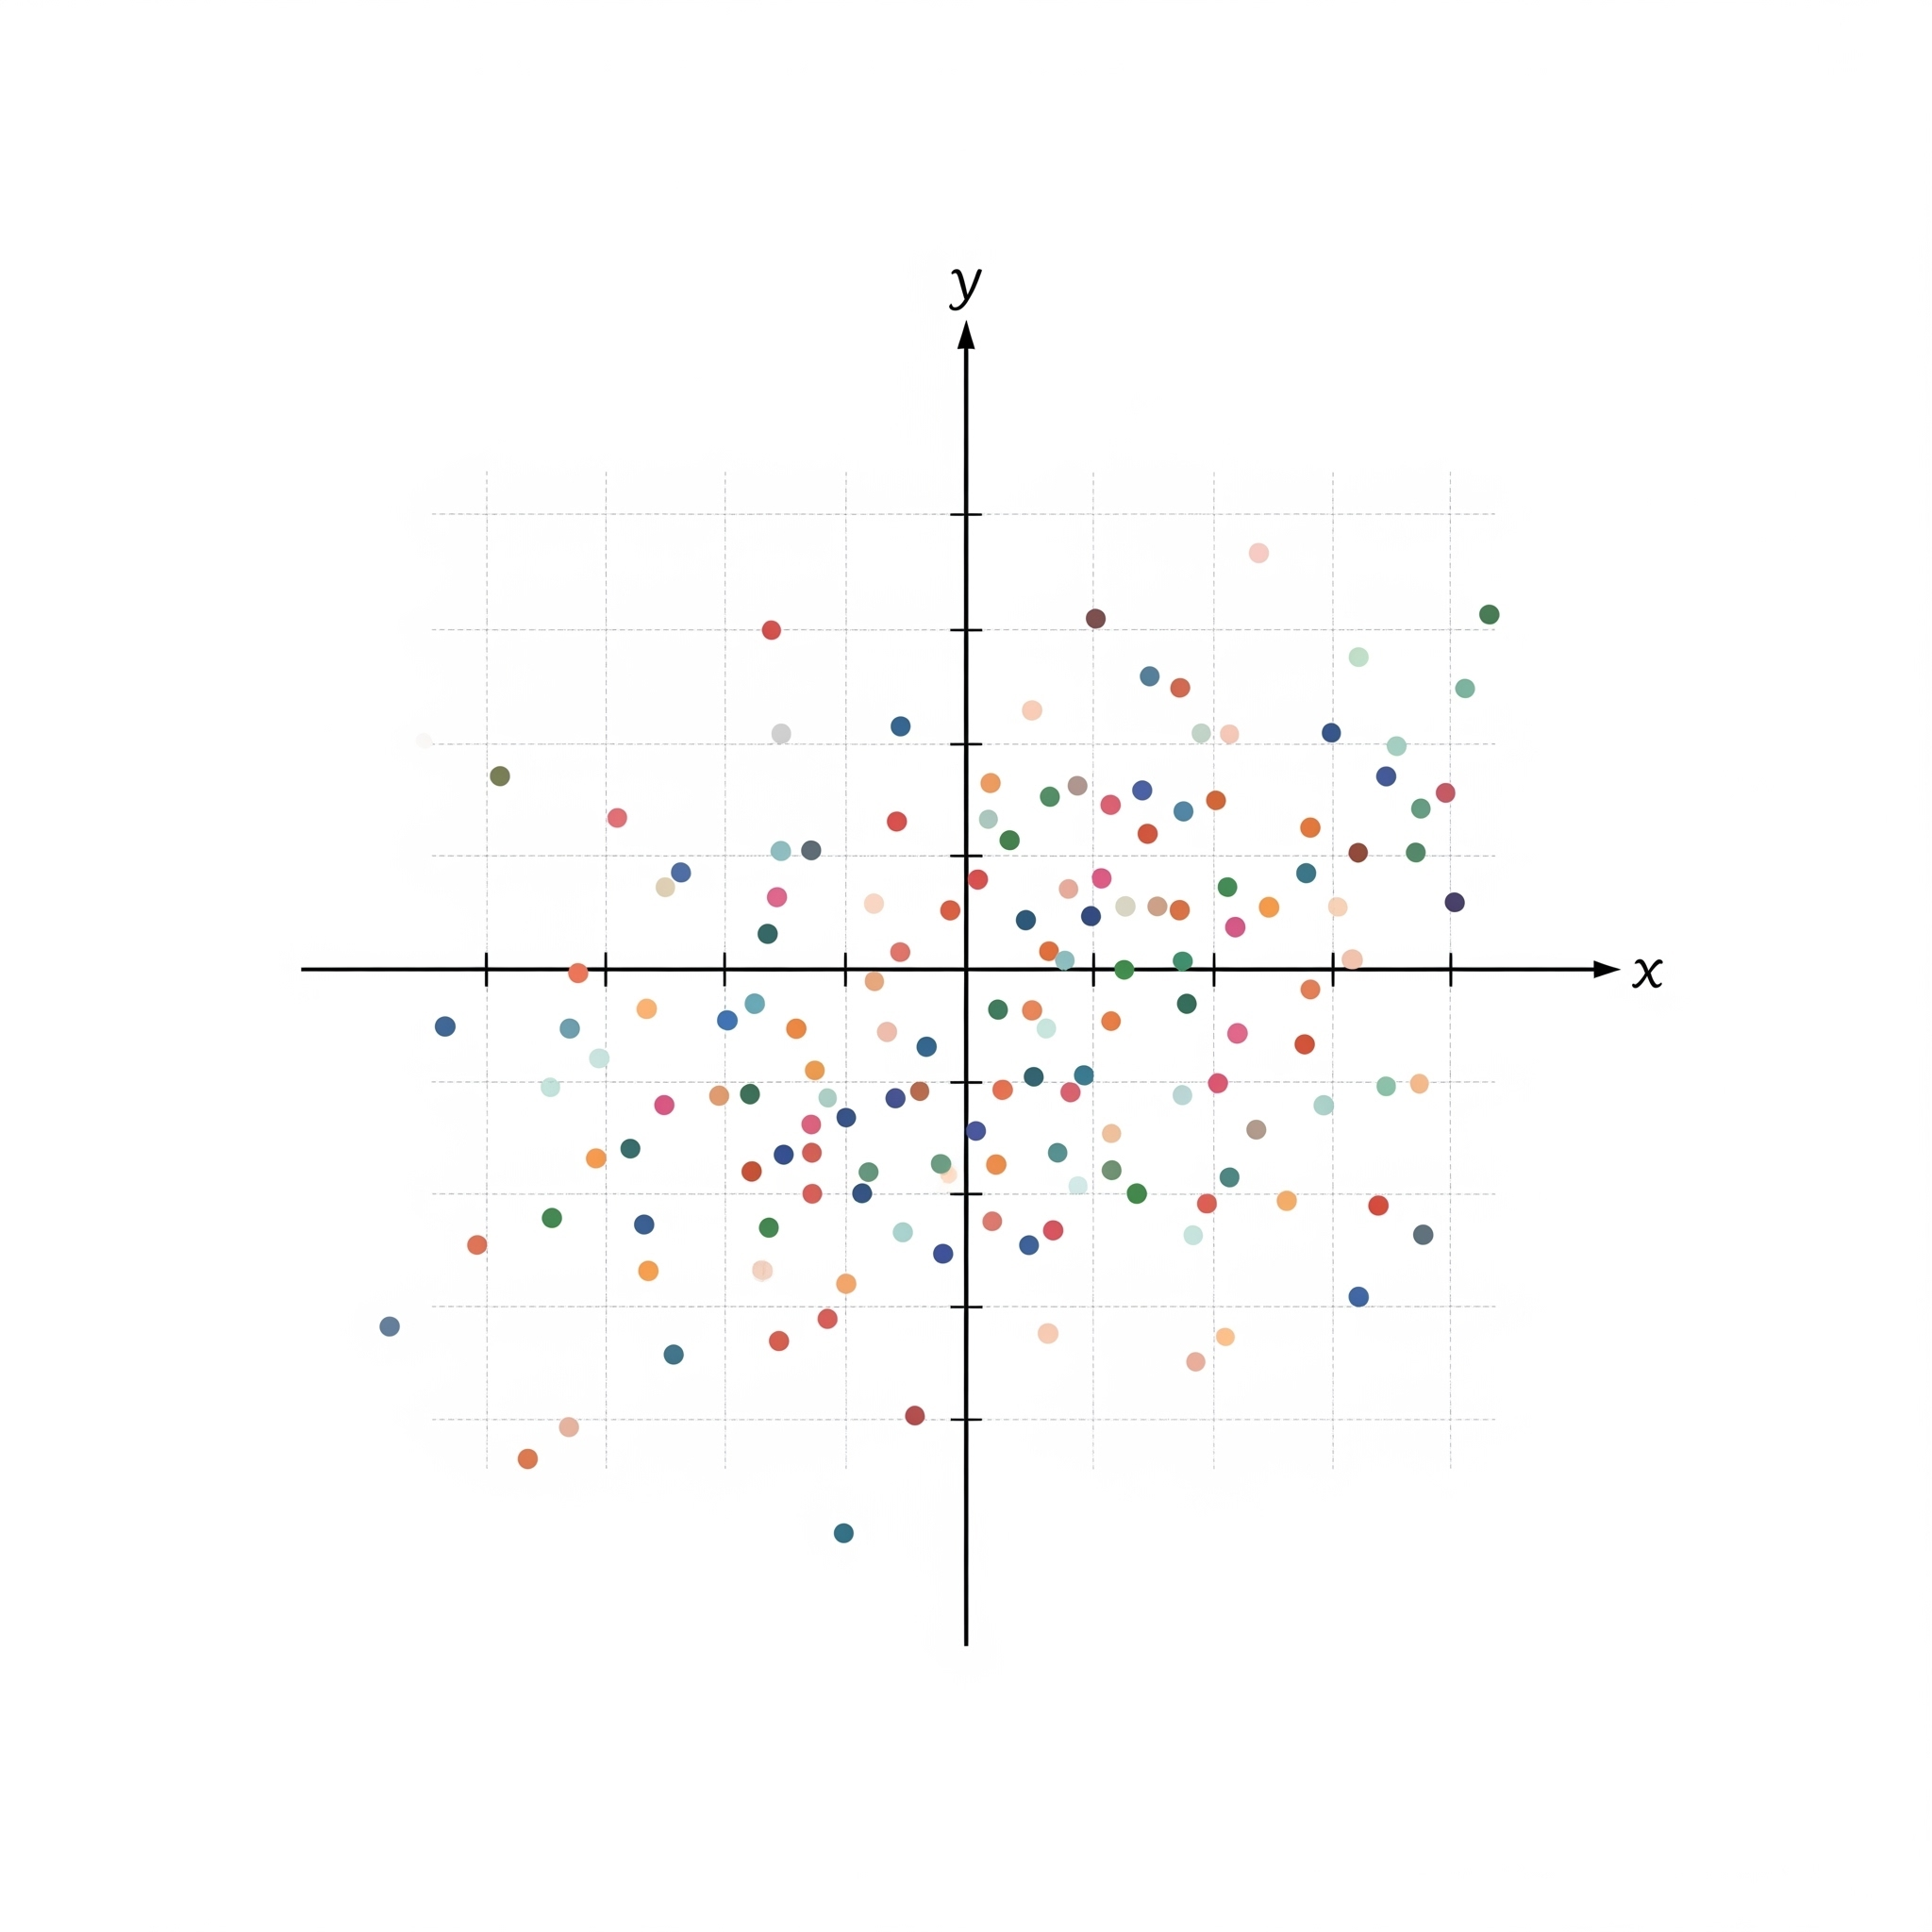
\includegraphics[width=0.8\textwidth]{data.png}
	
	% \caption provides the caption for your figure.
	% LaTeX will automatically number it (e.g., "Figure 1: My Data Plot").
	\caption{.}
	
	% \label creates a label for cross-referencing this figure in your text.
	% The 'fig:' prefix is a common convention.
	\label{fig:data_plot}
\end{figure}

\begin{figure}[htbp]
	% \centering command centers the image horizontally
	\centering
	
	% \includegraphics is the command to include the image.
	% [width=0.8\textwidth] scales the image to 80% of the text width.
	% You can adjust this value (e.g., 0.5\textwidth, or use height, or scale=0.7)
	% {data.png} is the filename. Ensure it's exact, including case.
	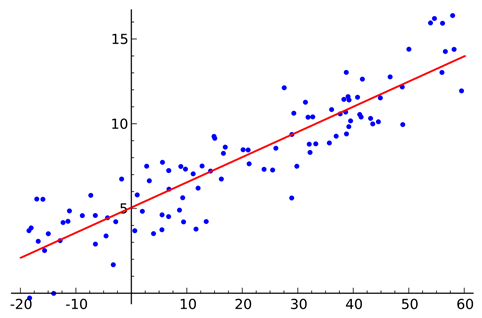
\includegraphics[width=0.8\textwidth]{lin-reg.png}
	
	% \caption provides the caption for your figure.
	% LaTeX will automatically number it (e.g., "Figure 1: My Data Plot").
	\caption{Datapoints lie almost along a straight line.}
	
	% \label creates a label for cross-referencing this figure in your text.
	% The 'fig:' prefix is a common convention.
	\label{fig:linreg_plot}
\end{figure}
\begin{figure}[htbp]
	% \centering command centers the image horizontally
	\centering
	
	% \includegraphics is the command to include the image.
	% [width=0.8\textwidth] scales the image to 80% of the text width.
	% You can adjust this value (e.g., 0.5\textwidth, or use height, or scale=0.7)
	% {data.png} is the filename. Ensure it's exact, including case.
	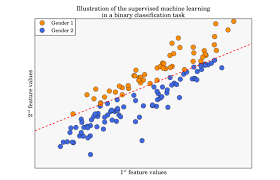
\includegraphics[width=0.8\textwidth]{log-reg.png}
	
	% \caption provides the caption for your figure.
	% LaTeX will automatically number it (e.g., "Figure 1: My Data Plot").
	\caption{Datapoints from 2 categories can be separated by a straight line.}
	
	% \label creates a label for cross-referencing this figure in your text.
	% The 'fig:' prefix is a common convention.
	\label{fig:logreg_plot}
\end{figure}

\end{document}
